\documentclass[12pt]{gshs_lecture}


\usepackage{framed}




%% Title, Author, Institute, Date %%
\title[]{\LaTeX\ for Beginner I}
\subtitle[]{GSHS \LaTeX\ Study}
\author[]{Chinook Mok}
\institute[GSHS]{Gyeonggi Science High School\\ for the gifted}
\date[]{\today}

%% Main %%
\begin{document}

%% Title page %%
\begin{frame}[plain]
\titlepage
\end{frame}
\setbeamertemplate{sidebar left}[sidebar theme]

\begin{frame}[t]{Outline}
\tableofcontents%[currentsection]
\end{frame}

\section{Why \LaTeX ?} %%%%%%%%%%%%%%%%%%%%%%%%%%%%%%%%%%%%%%%%%%%%%%%%%

\begin{frame}[t,fragile]{Why \LaTeX ?}\small
\vspace*{-1em}
\begin{itemize}
\item \textcolor{GSHSRED}{\textbf{Free:}} No cost to make and to view.
\item \textcolor{GSHSRED}{\textbf{PDF:}} Its result is the pdf format, the standard document granted by ISO.
\item \textcolor{GSHSRED}{\textbf{No mouse:}} You can make a document just by typing keyboard.
\item \textcolor{GSHSRED}{\textbf{Speed:}} The more proficient, therefore, the faster.
\item \textcolor{GSHSRED}{\textbf{Look:}} Nice and boundless mathematical formulas.
\item \textcolor{GSHSRED}{\textbf{Vector format:}} Images and graphs of a vector format (e.g. eps, pdf) keep their quality.
\item \textcolor{GSHSRED}{\textbf{Codebase:}} Fast conversion between papers and presentations.
\item \textcolor{GSHSRED}{\textbf{Unconstrained from OS:}}
\item \textcolor{GSHSRED}{\textbf{Light:}} Minimized GUI. Keyboard shortcuts are replaced by commands.
\item \textcolor{GSHSRED}{\textbf{WYSIWYM:}} Just writing text. Low computer resource. No lag.
\item \textcolor{GSHSRED}{\textbf{Automatic formation of ToC, LoF, LoT, Labels of equations, figures, and tables, ...}}
\end{itemize}
\end{frame}

\begin{frame}[t]{But...}\small
\begin{itemize}
\item \textcolor{GSHSRED}{\textbf{Unfamiliar:}} In general, one uses WYSIWYG style.
\item \textcolor{GSHSRED}{\textbf{Minimized GUI, Codebase:}} Higher entry barrier for beginner.
\item \textcolor{GSHSRED}{\textbf{Weak support for 한글}}
\end{itemize}
\par\vspace{5em}
\footnotesize\uncover<2->{\textbf{(Advantages of \LaTeX) $-$ (Disadvantages of \LaTeX)}}\uncover<3->{\textbf{=(POSITIVE)}}
\end{frame}

\section{Beginning \LaTeX} %%%%%%%%%%%%%%%%%%%%%%%%%%%%%%%%%%%%%%%%%%%%

\begin{frame}[t]{Outline}
\tableofcontents[currentsection]
\end{frame}

\begin{frame}[t,fragile]{Installing \LaTeX}\small
Install \LaTeX
\begin{itemize}
\item http://latex.gs.hs.kr/
\item https://namu.wiki/w/LaTeX
\end{itemize}
or you can use \LaTeX\ online
\begin{itemize}
\item https://ko.sharelatex.com/
\item https://www.overleaf.com/
\end{itemize}
\vspace{2em}
Hereafter this manual is written for the \LaTeX\ installed in your pc.
\end{frame}

\begin{frame}[t,fragile]{Make `*.tex' File}\small
Make a text file of the extension `tex'
\begin{center}
\begin{tikzpicture}
\draw (-0.05,0) rectangle (8,6.05);
\node[anchor=north west,inner sep=0] at (0,6) {\tiny {\textbackslash}documentclass[11pt]\{article\}};
\draw[GSHSRED,very thick,densely dashed,fill=gshsred] (0.5,4.7) rectangle (7.5,5.6) node[pos=0.5]{\Large Preamble};
\node[anchor=north west,inner sep=0] at (0,4.5) {\tiny {\textbackslash}begin\{document\}};
\draw[GSHSRED,very thick,densely dashed,fill=gshsred] (0.5,0.7) rectangle (7.5,4.1) node[pos=0.5]{\Large Body};
\node[anchor=north west,inner sep=0] at (0,0.5) {\tiny {\textbackslash}end\{document\}};
\end{tikzpicture}
\end{center}
\end{frame}

\begin{frame}[t,fragile]{Make `*.tex' File}\small
\begin{columns}[T]
\column{0.45\textwidth}
In the body,
\begin{block}{}
\begin{lstlisting}
She's gone
Out of my life
\end{lstlisting}
\end{block}
\column{0.45\textwidth}
then you have
\begin{block}{}
\textrm{She's gone Out of my life}
\end{block}
\end{columns}
\vspace{2em}
\begin{columns}[T]
\column{0.45\textwidth}
In the body,
\begin{block}{}
\begin{lstlisting}
She's gone

Out of my life
\end{lstlisting}
\end{block}
\column{0.45\textwidth}
you have
\begin{block}{}
\textrm{She's gone}\par
\textrm{Out of my life}
\end{block}
\end{columns}
\vspace{2em}
\begin{columns}[T]
\column{0.45\textwidth}
In the body,
\begin{block}{}
\begin{lstlisting}
She's gone\par
Out of my life
\end{lstlisting}
\end{block}
\column{0.45\textwidth}
you get
\begin{block}{}
\textrm{She's gone}\par
\textrm{Out of my life}
\end{block}
\end{columns}
\end{frame}

\section{Font} %%%%%%%%%%%%%%%%%%%%%%%%%%%%%%%%%%%%%%%%%%%%%%%%%%%%%%%

\begin{frame}[t]{Outline}
\tableofcontents[currentsection]
\end{frame}

\begin{frame}[t,fragile]{Font Size}\small
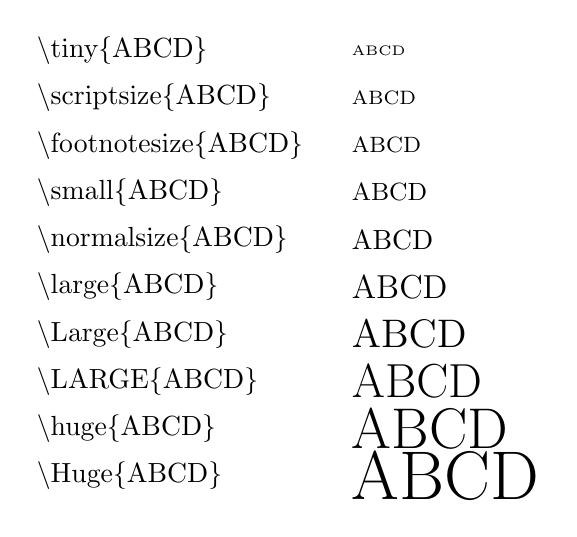
\begin{tikzpicture}
\node[anchor=west] at (0,5.4) {{\textbackslash}tiny\{ABCD\}};
\node[anchor=west] at (4,5.4) {\tiny ABCD};
\node[anchor=west] at (0,4.8) {{\textbackslash}scriptsize\{ABCD\}};
\node[anchor=west] at (4,4.8) {\scriptsize ABCD};
\node[anchor=west] at (0,4.2) {{\textbackslash}footnotesize\{ABCD\}};
\node[anchor=west] at (4,4.2) {\footnotesize ABCD};
\node[anchor=west] at (0,3.6) {{\textbackslash}small\{ABCD\}};
\node[anchor=west] at (4,3.6) {\small ABCD};
\node[anchor=west] at (0,3) {{\textbackslash}normalsize\{ABCD\}};
\node[anchor=west] at (4,3) {\normalsize ABCD};
\node[anchor=west] at (0,2.4) {{\textbackslash}large\{ABCD\}};
\node[anchor=west] at (4,2.4) {\large ABCD};
\node[anchor=west] at (0,1.8) {{\textbackslash}Large\{ABCD\}};
\node[anchor=west] at (4,1.8) {\Large ABCD};
\node[anchor=west] at (0,1.2) {{\textbackslash}LARGE\{ABCD\}};
\node[anchor=west] at (4,1.2) {\LARGE ABCD};
\node[anchor=west] at (0,0.6) {{\textbackslash}huge\{ABCD\}};
\node[anchor=west] at (4,0.6) {\huge ABCD};
\node[anchor=west] at (0,0) {{\textbackslash}Huge\{ABCD\}};
\node[anchor=west] at (4,0) {\Huge ABCD};
\end{tikzpicture}
\end{frame}

\begin{frame}[t,fragile]{Font Families}\small
Family
\begin{itemize}
\item \textrm{roman}  \textcolor{blue!70!black}{\texttt{{\textbackslash}textrm\{roman\}}}
\item \textsf{sans serif} \textcolor{blue!70!black}{\texttt{{\textbackslash}textsf\{sans serif\}}}
\item \texttt{typewriter} \textcolor{blue!70!black}{\texttt{{\textbackslash}texttt\{typewriter\}}}
\end{itemize}
Series
\begin{itemize}
\item \textrm{\textmd{medium}} \textcolor{blue!70!black}{\texttt{{\textbackslash}textmd\{medium\}}}
\item \textrm{\textbf{boldface}} \textcolor{blue!70!black}{\texttt{{\textbackslash}textbf\{boldface\}}}
\end{itemize}
Shape
\begin{itemize}
\item \textrm{upright}  \textcolor{blue!70!black}{\texttt{{\textbackslash}textup\{upright\}}}
\item \textrm{\textit{italic}} \textcolor{blue!70!black}{\texttt{{\textbackslash}textit\{italic\}}}
\item \textrm{\textsl{slanted}} \textcolor{blue!70!black}{\texttt{{\textbackslash}textsl\{slanted\}}}
\item \textrm{\textsc{small cap}} \textcolor{blue!70!black}{\texttt{{\textbackslash}textsc\{small cap\}}}
\end{itemize}
\end{frame}

\begin{frame}[t,fragile]{Times New Roman}\small
If you want to use `times new roman' font, write the following in the preamble
\begin{block}{}
\begin{lstlisting}
\usepackage{mathptmx}
\usepackage[T1]{fontenc} 
\usepackage[utf8]{inputenc}
\end{lstlisting}
\end{block}
\end{frame}

\section{Paragraph} %%%%%%%%%%%%%%%%%%%%%%%%%%%%%%%

\begin{frame}[t]{Outline}
\tableofcontents[currentsection]
\end{frame}

\begin{frame}[t,fragile]{Alignment}\small
In the body
\begin{block}{}
\begin{lstlisting}
\begin{center}
\LARGE\textbf{Why \LaTeX?}
\par\vspace{1em}
\large\textsf{GSHS \LaTeX\ Workshop 2018}
\end{center}
The default style of paragraph alignment is fully-justified paragraph. Copy and paste the previous sentence ten times here in order to make this paragraph longer.
\begin{flushleft}
The `flushleft' environment makes the paragraph the left-justified text. Again, copy and paste the previous sentence ten times here, to make this paragraph longer.
\end{flushleft}
\begin{flushright}
\textit{Chinook Mok}
\end{flushright}
\end{lstlisting}
\end{block}
\end{frame}

\begin{frame}[t]{Alignment}\small
you get
\begin{center}
\begin{framed}
\includegraphics[width=\textwidth,trim={1cm 18cm 1cm 4cm},clip]{./test_article/article001.pdf}

\end{framed}
\end{center}
\end{frame}


\section{Sections} %%%%%%%%%%%%%%%%%%%%%%%%%%%%%%%

\begin{frame}[t]{Outline}
\tableofcontents[currentsection]
\end{frame}

\begin{frame}[t,fragile]{Sections}\small
In the body,
\begin{block}{}
\begin{lstlisting}
\section{She's Gone}

She's gone out of my life. I was wrong, I'm to blame, I was so untrue, I can't live without her love. In my life there's just an empty space. All my dreams are lost. I'm wasting away. Forgive me, girl. Lady, won't you save me? My heart belongs to you. Lady, can you forgive me? For all I've done to you. Lady, oh, lady.

\section{Bohemian Rhapsody}

Is this the real life? Is this just fantasy? Caught in a landslide. No escape from reality. Open your eyes. Look up to the skies and see. I'm just a poor boy, I need no sympathy. Because I'm easy come, easy go, a little high, little low. Anyway the wind blows, doesn't really matters to me, to me.
\end{lstlisting}
\end{block}
\end{frame}

\begin{frame}[t]{Sections}\small
you get
\begin{center}
\begin{framed}
\includegraphics[width=\textwidth,trim={1cm 18cm 1cm 4cm},clip]{./test_article/article002.pdf}
\end{framed}
\end{center}
\end{frame}

\begin{frame}[t,fragile]{Subsections}\small
In the body,
\begin{block}{}
\begin{lstlisting}
\section{She's Gone}

She's gone out of my life. I was wrong, I'm to blame, I was so untrue, I can't live without her love. In my life there's just an empty space. All my dreams are lost. I'm wasting away. Forgive me, girl. Lady, won't you save me? My heart belongs to you. Lady, can you forgive me? For all I've done to you. Lady, oh, lady.

\subsection{Bohemian Rhapsody}

Is this the real life? Is this just fantasy? Caught in a landslide. No escape from reality. Open your eyes. Look up to the skies and see. I'm just a poor boy, I need no sympathy. Because I'm easy come, easy go, a little high, little low. Anyway the wind blows, doesn't really matters to me, to me.
\end{lstlisting}
\end{block}
\end{frame}

\begin{frame}[t]{Subsections}\small
you get
\begin{center}
\begin{framed}
\includegraphics[width=\textwidth,trim={1cm 18cm 1cm 4cm},clip]{./test_article/article003.pdf}
\end{framed}
\end{center}
\end{frame}

\begin{frame}[t,fragile]{Section---Modification}\small
In the preamble,
\begin{block}{}
\begin{lstlisting}
\usepackage{secdot}
\sectiondot{subsection}
\end{lstlisting}
\end{block}
then you get
\begin{center}
\begin{framed}
\includegraphics[width=0.7\textwidth,trim={1cm 18cm 1cm 4cm},clip]{./test_article/article004.pdf}
\end{framed}
\end{center}
\end{frame}


\begin{frame}[t,fragile]{Section---Modification}\small
In the preamble,
\begin{block}{}
\begin{lstlisting}
\renewcommand{\thesection}{\Roman{section}}
\renewcommand{\thesubsection}{\thesection.\roman{subsection}}
\end{lstlisting}
\end{block}
then you get
\begin{center}
\begin{framed}
\includegraphics[width=0.7\textwidth,trim={0cm 18cm 0cm 4cm},clip]{./test_article/article005.pdf}
\end{framed}
\end{center}
\end{frame}

\begin{frame}[t,fragile]{Section---Reference}\small
In the body,
\begin{block}{}
\begin{lstlisting}
\section{She's Gone}\label{sec:shes_gone}

She's gone out of my life. I was wrong, I'm to blame, I was so untrue, I can't live without her love. In my life there's just an empty space. All my dreams are lost. I'm wasting away. Forgive me, girl. Lady, won't you save me? My heart belongs to you. Lady, can you forgive me? For all I've done to you. Lady, oh, lady. In the section \ref{sec:bohemian} we'll meet `\emph{Queen}'!

\section{Bohemian Rhapsody}\label{sec:bohemian}

Is this the real life? Is this just fantasy? Caught in a landslide. No escape from reality. Open your eyes. Look up to the skies and see. I'm just a poor boy, I need no sympathy. Because I'm easy come, easy go, a little high, little low. Anyway the wind blows, doesn't really matters to me, to me. In the section \ref{sec:shes_gone}, we had met `\emph{Steel Heart}'!
\end{lstlisting}
\end{block}
\end{frame}

\begin{frame}[t]{Section---Reference}\small
then you get
\begin{center}
\begin{framed}
\includegraphics[width=0.7\textwidth,trim={0cm 16cm 0cm 4cm},clip]{./test_article/article006.pdf}
\end{framed}
\end{center}
\end{frame}

\section{Title} %%%%%%%%%%%%%%%%%%%%%%%%%%%%%%%%%%%%%%%%%%%%%%%%%%%

\begin{frame}[t]{Outline}
\tableofcontents[currentsection]
\end{frame}

\begin{frame}[t,fragile]{Title}\small
In the preamble,
\begin{block}{}
\begin{lstlisting}
\title{\textbf{Let's Sing!}}
\author{Chinook Mok}
\date{\small\today}
\end{lstlisting}
\end{block}
In the body,
\begin{block}{}
\begin{lstlisting}
\maketitle
\end{lstlisting}
\end{block}
\end{frame}

\begin{frame}[t]{Title}\small
you get
\begin{center}
\begin{framed}
\includegraphics[width=\textwidth,trim={0cm 13cm 0cm 4cm},clip]{./test_article/article007.pdf}
\end{framed}
\end{center}
\end{frame}

\begin{frame}[t,fragile]{Title---Affiliation}\small
In the preamble,
\begin{block}{}
\begin{lstlisting}
\usepackage{authblk}

\title{\textbf{Let's Sing!}}
\author{Chinook Mok}
\affil{GSHS}
\author{Sowon}
\author{Yerin}
\author{Yuju}
\affil{GFRIEND}
\date{\small\today}
\end{lstlisting}
\end{block}
In the body,
\begin{block}{}
\begin{lstlisting}
\maketitle
\end{lstlisting}
\end{block}
\end{frame}

\begin{frame}[t]{Title---Affiliation}\small
you get
\begin{center}
\begin{framed}
\includegraphics[width=\textwidth,trim={0cm 13cm 0cm 4cm},clip]{./test_article/article008.pdf}
\end{framed}
\end{center}
\end{frame}

\section{Equations} %%%%%%%%%%%%%%%%%%%%%%%%%%%%%%%%%%%%%%%%%

\begin{frame}[t]{Outline}
\tableofcontents[currentsection]
\end{frame}

\begin{frame}[t,fragile]{Equations---Single line}\small
In the preamble,
\begin{block}{}
\begin{lstlisting}
\usepackage{amsmath}
\end{lstlisting}
\end{block}
In the body,
\begin{block}{}
\begin{lstlisting}
Two objects of mass $m_1$ and $m_2$ are located at $\mathbf{r}_1$ and $\mathbf{r}_2$, respectively. The force exerted on the body of $m_1$ due to that of $m_2$ is given by
\begin{equation}
\mathbf{F}_{12} =-G\frac{m_1 m_2}{r^2}\hat{\mathbf{r}}_{12}.\label{eq:grav_force}
\end{equation}
where $G\approx (20/3)\times 10^{-11}\,\mathrm{m^3 kg^{-1}s^{-2}}$ is the universal gravitational constant, $r=|\mathbf{r}_1 -\mathbf{r}_2 |$ is the distance from $m_2$ to $m_1$, and $\hat{\mathbf{r}}_{12}$ is the unit vector of $\mathbf{r}_{12} \equiv\mathbf{r}_1 -\mathbf{r}_2$.
\end{lstlisting}
\end{block}
\end{frame}

\begin{frame}[t]{Equations---Single line}\small
you get
\begin{center}
\begin{framed}
\includegraphics[width=\textwidth,trim={0cm 18cm 0cm 4cm},clip]{./test_article/article009.pdf}
\end{framed}
\end{center}
\end{frame}

\begin{frame}[t,fragile]{Equations---Multi lines}\small
In the body,
\begin{block}{}
\begin{lstlisting}
\begin{equation}
\begin{split}
\frac{d\omega_b^2}{dt}=(\gamma_L -\gamma_d )\omega_b^2 &-\frac{\gamma_L}{2}\int_{t/2}^t dt_1 \int_{t-t_1}^{t_1} dt_2 (t-t_1 )^2 \\
& e^{-\nu_a (2t-t_1 -t_2 )} \omega_b^2 (t_1)\omega_b^2(t_2)\omega_b^2(t+t_2 -t_1).
\end{split}
\label{eq:BBmodel}
\end{equation}
\end{lstlisting}
\end{block}
we get
\begin{center}
\begin{framed}
\includegraphics[width=\textwidth,trim={0cm 22cm 0cm 4.6cm},clip]{./test_article/article010.pdf}
\end{framed}
\end{center}
\end{frame}

\begin{frame}[t,fragile]{Equations---Multi lines}\small
In the body,
\begin{block}{}
\begin{lstlisting}
\begin{align}
\oint_S \mathbf{E}\cdot d\mathbf{A} &=\int_V \frac{\rho}{\epsilon_0}\mathrm{d}V \label{eq:Gauss}\\
\oint_S \mathbf{B}\cdot d\mathbf{A} &=0 \label{eq:No_Monopole_B}\\
\oint_C \mathbf{E}\cdot d\mathbf{l} &=-\frac{\partial}{\partial t}\int_S \mathbf{B}\cdot\mathrm{d}\mathbf{A} \label{eq:Faraday}\\
\oint_C \mathbf{B}\cdot d\mathbf{\mathcal{l}} &=\mu_0 \int_S \mathbf{J}\cdot\mathrm{d}\mathbf{A}+\mu_0 \epsilon_0 \frac{\partial}{\partial t}\int_S \mathbf{E}\cdot\mathrm{d}\mathbf{A} \label{eq:Ampere}
\end{align}
\end{lstlisting}
\end{block}
we get
\begin{center}
\begin{framed}
\includegraphics[width=\textwidth,trim={0cm 20.2cm 0cm 5.2cm},clip]{./test_article/article011.pdf}
\end{framed}
\end{center}
\end{frame}

\begin{frame}[t,fragile]{Equations---Reference}\small
In the body,
\begin{block}{}
\begin{lstlisting}
\begin{equation}
\mathbf{F} =-G\frac{m_1 m_2}{r^2}\hat{\mathbf{r}}.\label{eq:grav_force}
\end{equation}
Dividing both sides of \eqref{eq:grav_force} by $m_1$ we obtain the gravitational field due to $m_2$.
\end{lstlisting}
\end{block}
we get
\begin{center}
\begin{framed}
\includegraphics[width=\textwidth,trim={0cm 21.5cm 0cm 4cm},clip]{./test_article/article012.pdf}
\end{framed}
\end{center}
\end{frame}

\section{Figures} %%%%%%%%%%%%%%%%%%%%%%%%%%%%%%%%%%%%%%%%%%%%%%%%%%%

\begin{frame}[t]{Outline}
\tableofcontents[currentsection]
\end{frame}

\begin{frame}[t]{Vector Image and Raster Image}\small
\begin{center}
\includegraphics[width=0.4\textwidth]{./figures/vector_image.pdf}\hspace{2em}
\includegraphics[width=0.4\textwidth]{./figures/raster_image.png}
\end{center}
\begin{columns}[T]
\column{0.45\textwidth}
\begin{itemize}
\item \textbf{PDF}
\item PS
\item EPS
\end{itemize}
\column{0.45\textwidth}
\begin{itemize}
\item \textbf{PNG}
\item JPEG
\end{itemize}
\end{columns}
\end{frame}

\begin{frame}[t,fragile]{Import an Image File}\small
You should have a figure file above all. If the path of the figure file is, e.g., `./figures/graph.pdf', write following in the preamble,
\begin{block}{}
\begin{lstlisting}
\usepackage{graphicx}
\end{lstlisting}
\end{block}
and in the body,
\begin{block}{}
\begin{lstlisting}
\includegraphics[width=0.5\textwidth]{./figures/graph.pdf}
\end{lstlisting}
\end{block}
we get
\begin{center}
\begin{framed}
\includegraphics[width=\textwidth,trim={0cm 20cm 0cm 4cm},clip]{./test_article/article013.pdf}
\end{framed}
\end{center}
\end{frame}

\begin{frame}[t,fragile]{Figure Environment}\small
In the body,
\begin{block}{}
\begin{lstlisting}
\begin{figure}[t]
\centering
\includegraphics[width=0.5\textwidth]{./figures/graph.pdf}
\caption{Number of beads in every tubes spaced at regular intervals.}
\label{fig:result01}
\end{figure}
\end{lstlisting}
\end{block}
we get
\begin{center}
\begin{framed}
\includegraphics[width=\textwidth,trim={0cm 11cm 0cm 10cm},clip]{./test_article/article014.pdf}
\end{framed}
\end{center}
\end{frame}

\begin{frame}[t,fragile]{Figure Environment}\small
The option of the figure environment specifies the placement.
\begin{itemize}
\item \textcolor{GSHSRED}{\textbf{h}} Place the float \emph{here}.
\item \textcolor{GSHSRED}{\textbf{t}} Position at the \emph{top} of the page.
\item \textcolor{GSHSRED}{\textbf{b}} Position at the \emph{bottom} of the page.
\item \textcolor{GSHSRED}{\textbf{p}} Put on a special \emph{page} for floats only.
\end{itemize}
\begin{block}{}
\begin{lstlisting}
\usepackage[labelsep=period,labelfont=bf]{caption}
\end{lstlisting}
\end{block}
makes \textrm{Figure 1:} $\rightarrow$ \textbf{\textrm{Figure 1.}}
\begin{block}{}
\begin{lstlisting}
\renewcommand{\figurename}{Fig}
\end{lstlisting}
\end{block}
makes \textbf{\textrm{Fig 1.}}
\end{frame}

\section{Further Subjects} %%%%%%%%%%%%%%%%%%%%%%%%%%%%%%%%%%%%%%%%%%%

\begin{frame}[t]{In the next time ...}\small
\begin{itemize}
\item \textcolor{GSHSRED}{\textbf{Table}}
\item \textcolor{GSHSRED}{\textbf{Itemization}}
\item \textcolor{GSHSRED}{\textbf{Citation}}
\item \textcolor{GSHSRED}{\textbf{Header and Footer}}
\item \textcolor{GSHSRED}{\textbf{Document Class}}
\item \textcolor{GSHSRED}{\textbf{Beamer}}
\end{itemize}
\vspace*{1.6em}
\emph{Expert}
\begin{itemize}
\item \textcolor{GSHSRED}{\textbf{TikZ}}
\begin{itemize}
\item Basic: 2D drawing
\item sub-packages: circuitikz, tikz-3dplot
\end{itemize}
\end{itemize}
\end{frame}








\end{document}